\section{Procédés de fabrication des MID}
Il existe actuellement 2 méthodes de production de \textsc{mid} sur le marché :
le \emph{Laser Direct Structuring} et le \emph{Two-shot molding}. Le premier est
de loin le plus répandu (environ 80\% du marché selon \cite{mid-2011}), car moins
cher et plus adapté aux petites séries, tandis que le second est utilisé lorsque
la géométrie de la pièce ne permet pas l'usage du \textsc{lds}.

\subsection{Laser Direct Structuring}
\begin{figure}[h]
    \begin{center}
        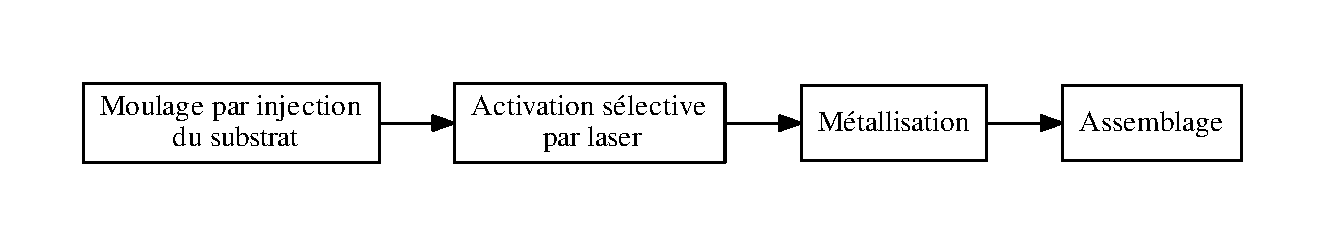
\includegraphics[width=\textwidth]{images/lds_process}
        \caption{Vue d'ensemble du processus \emph{Laser Direct Structuring}}\label{fig:lds-process}
    \end{center}
\end{figure}
Le \textsc{lds} est un procédé relativement récent, ayant été introduit sur le
marché en 2006. Par conséquent, c'est une technologie brevetée de LPKF Lasers \&
Electronics AG en Allemagne. Leur site web\footnote{\url{www.lpkf.com}} est donc
une excellente source d'informations pour la conception de pièces utilisant
le \textsc{lds-mid}.

\subsubsection{Principe de base du procédé}
Le principe général du procédé est visible à la fig. \ref{fig:lds-process}. On
retrouve donc, dans l'ordre :

\begin{description}
    \item[Injection] Moulage par injection d'un thermoplastique. Le détail de cette étape
        sort du cadre de ce séminaire. On se référera à celui sur l'injection
        plastique. 
    \item[Activation] Le polymère ayant servi pour l'injection de la pièce a
        préalablement été
        dopé avec un composant organométallique qui est activé par le laser en
        suivant le tracé des pistes voulues. Une réaction physique décompose
        alors ce dopant entre partie métallique et partie organique.
        Les lasers utilisés sont typiquement des lasers infra-rouges d'une
    \item[Métallisation] L'étape de métallisation commence par une étape de
        nettoyage, afin de faciliter l'accrochage. Les pistes sont ensuites
        construites par dépose de fine couches (environ \SI{5}{\micro\meter}).
        Finalement, un traitement de surface contre l'oxydation est appliqué. Ce
        traitement consiste généralement en une couche de nickel suivi d'une
        couche d'or, mais des traitements spécifiques, à base d'étain ou
        d'argent sont également possibles.
    \item[Assemblage] Les composants électriques annexes (boutons, connecteurs,
        etc\ldots) sont soudés sur le \textsc{mid}. Pendant le prototypage cette
        étape est souvent faite à la main, avec un fer à souder. Pour la
        production, si le polymère a une température de fusion suffisament
        élevée, l'assemblage par \emph{reflow soldering} est utilisable. 
\end{description}
